\documentclass[10pt]{beamer}

\usetheme[progressbar=frametitle]{metropolis}
\usepackage{mathtools}
\usepackage{amsmath}
\usepackage{booktabs}
\usepackage[scale=2]{ccicons}

\usepackage{pgfplots}
\usepgfplotslibrary{dateplot}
\usepackage{graphicx}
\graphicspath{}
 

\DeclareMathOperator*{\argmaxA}{arg\,max} % Jan Hlavacek
\DeclareMathOperator*{\argminB}{argmin}   % Jan Hlavacek
\DeclareMathOperator*{\argminC}{\arg\min}   % rbp

\newcommand{\argminD}{\arg\!\min} % AlfC

\newcommand{\argminE}{\mathop{\mathrm{argmin}}}          % ASdeL
\newcommand{\argminF}{\mathop{\mathrm{argmin}}\limits}   % ASdeL

\usepackage{xspace}
\newcommand{\themename}{\textbf{\textsc{metropolis}}\xspace}
% A Segment-Based Feature Measure For Capturing Repetitive Structures Of Music Recordings
\title{
Processamento e identificação automática de cantos de pássaros
}
\subtitle{}
\date{\today}
\author{Felipe Felix $(f^2)$}
\institute{IME-USP}
%\titlegraphic{\hfill
\includegraphics[height=1.5cm]{logo}}

\begin{document}

\maketitle

\begin{frame}{Table of contents}
  \setbeamertemplate{section in toc}[sections numbered]
  \tableofcontents[hideallsubsections]
\end{frame}

\section{Introduction}

\begin{frame}[fragile]{Introduction}
\begin{itemize}
\item Automatic identification and classification system for bird species using their sounds.
\item Estimation of the range, population size, 
and population trends using ARUs.
\item Biodiversity indicators.
\end{itemize}
\end{frame}

\begin{frame}[fragile]{Audio classification general structure}

\begin{figure}[h]
%\centering
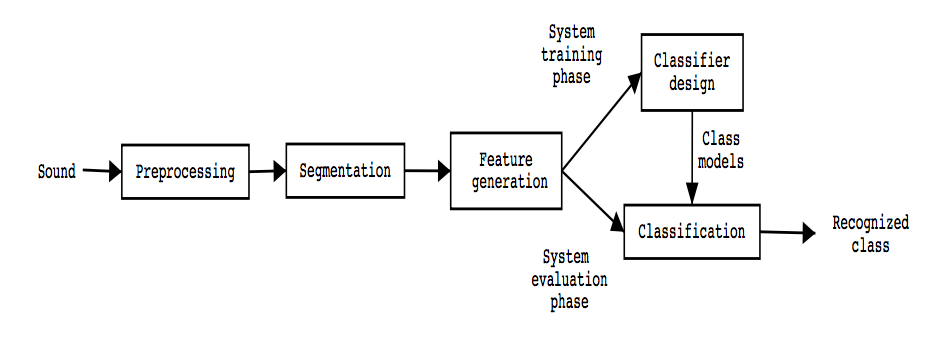
\includegraphics[width=1\textwidth]{estrutura}
\end{figure}


\end{frame}


\begin{frame}[fragile]{Introduction - Bird Sounds}
\begin{itemize}
\item Usually divided in three categories: \textit{call}, \textit{song}, \textit{mechanical sounds}.
\item $Calls$ usually refer to simple frequency 
patterns of short  monosyllabic sounds. 
\item  $Songs$ are longer than calls,  acoustically more complex, and often have a modular  structure.
\item  Hierarchical levels of bird  song: phrases,
syllables,  and elements (or notes).
\item  \textit{Element}  is the smallest  separable  element
in  spectrogram.
\item  \textit{Syllables} are produced  by one or more elements.
\item Series of \textit{syllables} that occur  together in a particular pattern is called a \textit{phrase}.

\end{itemize}
\end{frame}

\begin{frame}{Example}
\begin{figure}[h]
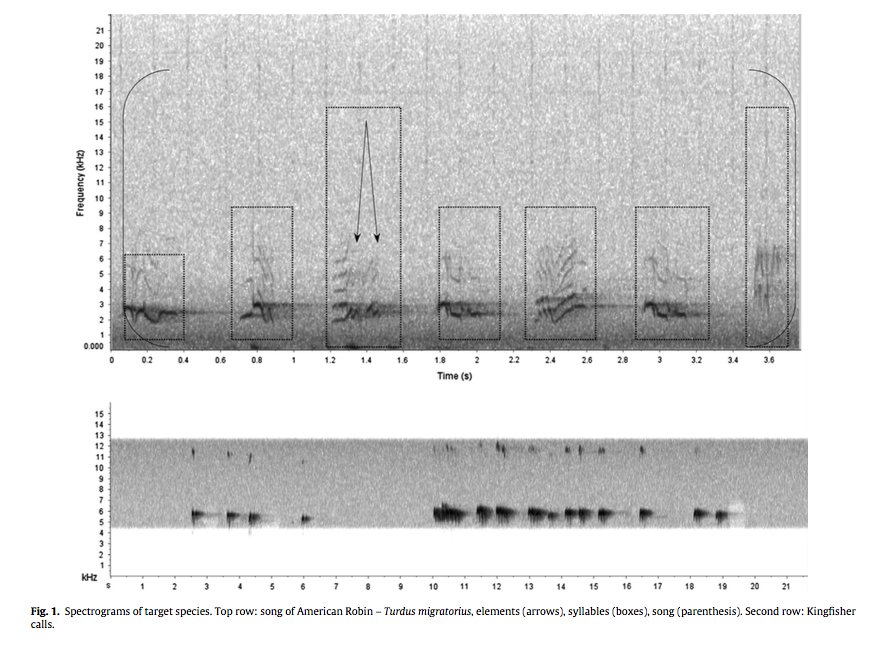
\includegraphics[width=1\textwidth]{song_call}
\end{figure}
\end{frame}

\begin{frame}[fragile]{Example}
\begin{figure}
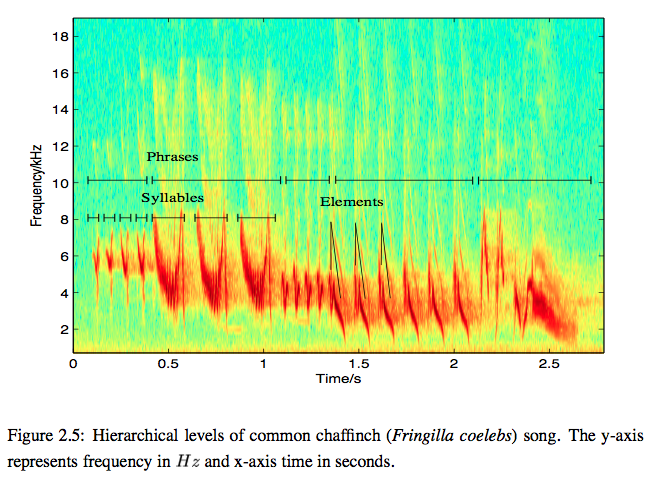
\includegraphics[width=1\textwidth]{structure}
\end{figure}
\end{frame}



\section{Segmentation Algorithm}

\begin{frame}[fragile]{Algorithm}
\begin{itemize}
\item Based on the energy of audio file and the noise level estimate.
\item \textbf{First phase}: onset and offset of the syllable candidates are calculated.
\item Near onset and offset areas of syllable candidates energy envelope  curve commonly fluctuates around the threshold, which causes short
erroneous candidates (\textit{border effect}).
\item \textbf{Second phase}: syllable candidates enough close to each other in temporal domain are connected to a single syllable.
\item \textbf{Last phase}: true syllable detection; where too short candidates are omitted.	
\end{itemize}
\end{frame}


\begin{frame}[fragile]{Onset/Offset detection}
\begin{itemize}
\item File is divided into the overlapping frames.
\item Frames are windowed using the hanning window.
\item The energy envelope $E(m)$ of the signal $x(n)$ in decibel scale is calculated as
\begin{equation}
E(m) = \sum\limits_{i=1}^{N} 20log_{10}|x_i[n]|^2
\end{equation}
where $x_i[n]$ is $i$:th frame and $N$ is the total number of frames of the signal $x(n)$ (?).
\end{itemize}
\end{frame}

\begin{frame}[fragile]{Flow diagram of syllable search algorithm}
\begin{figure}
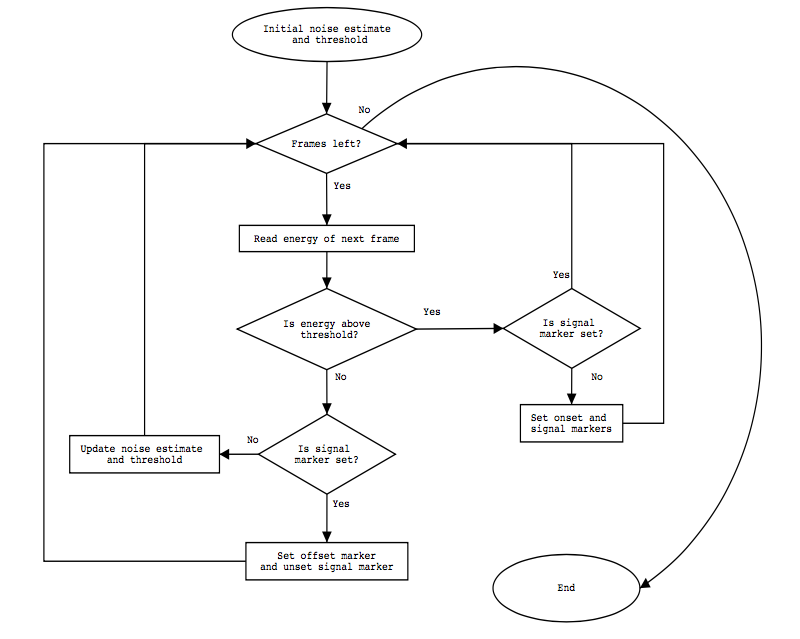
\includegraphics[width=0.95\textwidth]{flow}
\end{figure}
\end{frame}

\begin{frame}[fragile]{Example}
\begin{figure}
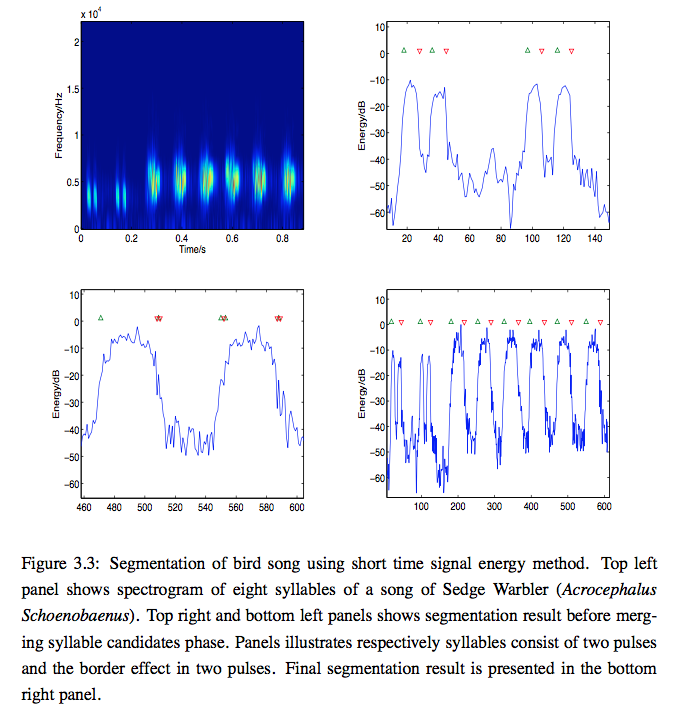
\includegraphics[width=0.73\textwidth]{example2}
\end{figure}
\end{frame}

\begin{frame}[fragile]{References}
[1] Potamitis, Ilyas, et al. "Automatic bird sound detection in long real-field recordings: Applications and tools." Applied Acoustics 80 (2014): 1-9.\\

[2] Fagerlund, Seppo. Automatic recognition of bird species by their sounds. Diss. Helsinki University of technology, 2004.
\end{frame}
\end{document}

%
% nmf tem se tornado popular pra separação de fontes musicais, mas lida apenas com a magnitude do espectrograma, e descarta a fase
% 
% o espectrograma dos componentes são estimados usando um filtro Wiener que reusa as fases do espectrograma original
% 
% mas é dificil recuperar fontes de áudio de alta qualidade pq o espectrograma original é inconsistente
% 
% pra evitar a reconstrução de fase no dominio da frequencia, eles usam o PSDTF pra estimar as fontes direto no dominio do tempo
% 
% PSDTF é uma extensão do NMF
% 
% ====
% 
% NMF - aproximar uma matrix não negativa da eergia do espectrograma de um sinal misto como sendo o produto de outras duas matrizes nao negativas, % sendo uma um conjunto de spectros de base e outra  uma matriz de ativação% 
% 
% decomposição do sinal misto em uma soma de espectrogramas de origem, usando filtro wiener
% 
% 
% 
% ===================
% 
% 1. fontes de audio originais usadas pelo autor
% 2. fontes novas
% 	- melhorar a qualidade (gravar de verdade)
% 	- fazer o treinamento mudando os inicios
% 	- som ruidosos
% 	- voz
% 	- mais Ks (4, 5?)
% 